\documentclass[12pt]{article}
\usepackage[utf8]{inputenc}
\usepackage[spanish]{babel}
\usepackage{graphicx}
\usepackage{amsmath}
\usepackage{amssymb}
\usepackage{array}
\usepackage{xcolor}
\usepackage{geometry}
\usepackage{fancyhdr}
\usepackage{lastpage}
\usepackage{booktabs}
\usepackage{colortbl}
\usepackage{caption}
\usepackage{multirow}
\geometry{margin=1in}

\usepackage{float}
\definecolor{lightblue}{RGB}{200,230,255}
\definecolor{lightgreen}{RGB}{220,255,220}
\definecolor{lightred}{RGB}{255,220,220}
\definecolor{lightyellow}{RGB}{255,255,200}
\pagestyle{fancy}
\fancyhf{}
\fancyhead[L]{Algoritmo de Floyd - Solución}
\fancyhead[R]{\thepage\ de \pageref{LastPage}}
\renewcommand{\headrulewidth}{0.4pt}
\renewcommand{\footrulewidth}{0.4pt}

\title{Proyecto 1: Rutas Optimas (Algoritmo de Floyd)}
\author{Emily Sanchez \\ Viviana Vargas \\[1cm] Curso: Investigación de Operaciones \\ II Semestre 2025}
\date{\today}

\begin{document}

\maketitle
\thispagestyle{empty}
\newpage
\setcounter{page}{1}

\section{Introducción}
El algoritmo de Floyd-Warshall es un algoritmo para encontrar los caminos más cortos en un grafo ponderado. Fue publicado por Robert Floyd en 1962.\\
El algoritmo de Floyd se basa en el principio de la Programación Dinámica.\\
\textbf{Complejidad espacial:} $O(n^2)$\\
\textbf{Complejidad temporal:} $O(n^3)$\\
\clearpage
\section{Descripción del Problema}
Grafo con 9 nodos:

\begin{itemize}
\item Nodo A: A
\item Nodo B: B
\item Nodo C: C
\item Nodo D: D
\item Nodo E: E
\item Nodo F: F
\item Nodo G: G
\item Nodo H: H
\item Nodo I: I
\end{itemize}

\begin{figure}[h!]
\centering
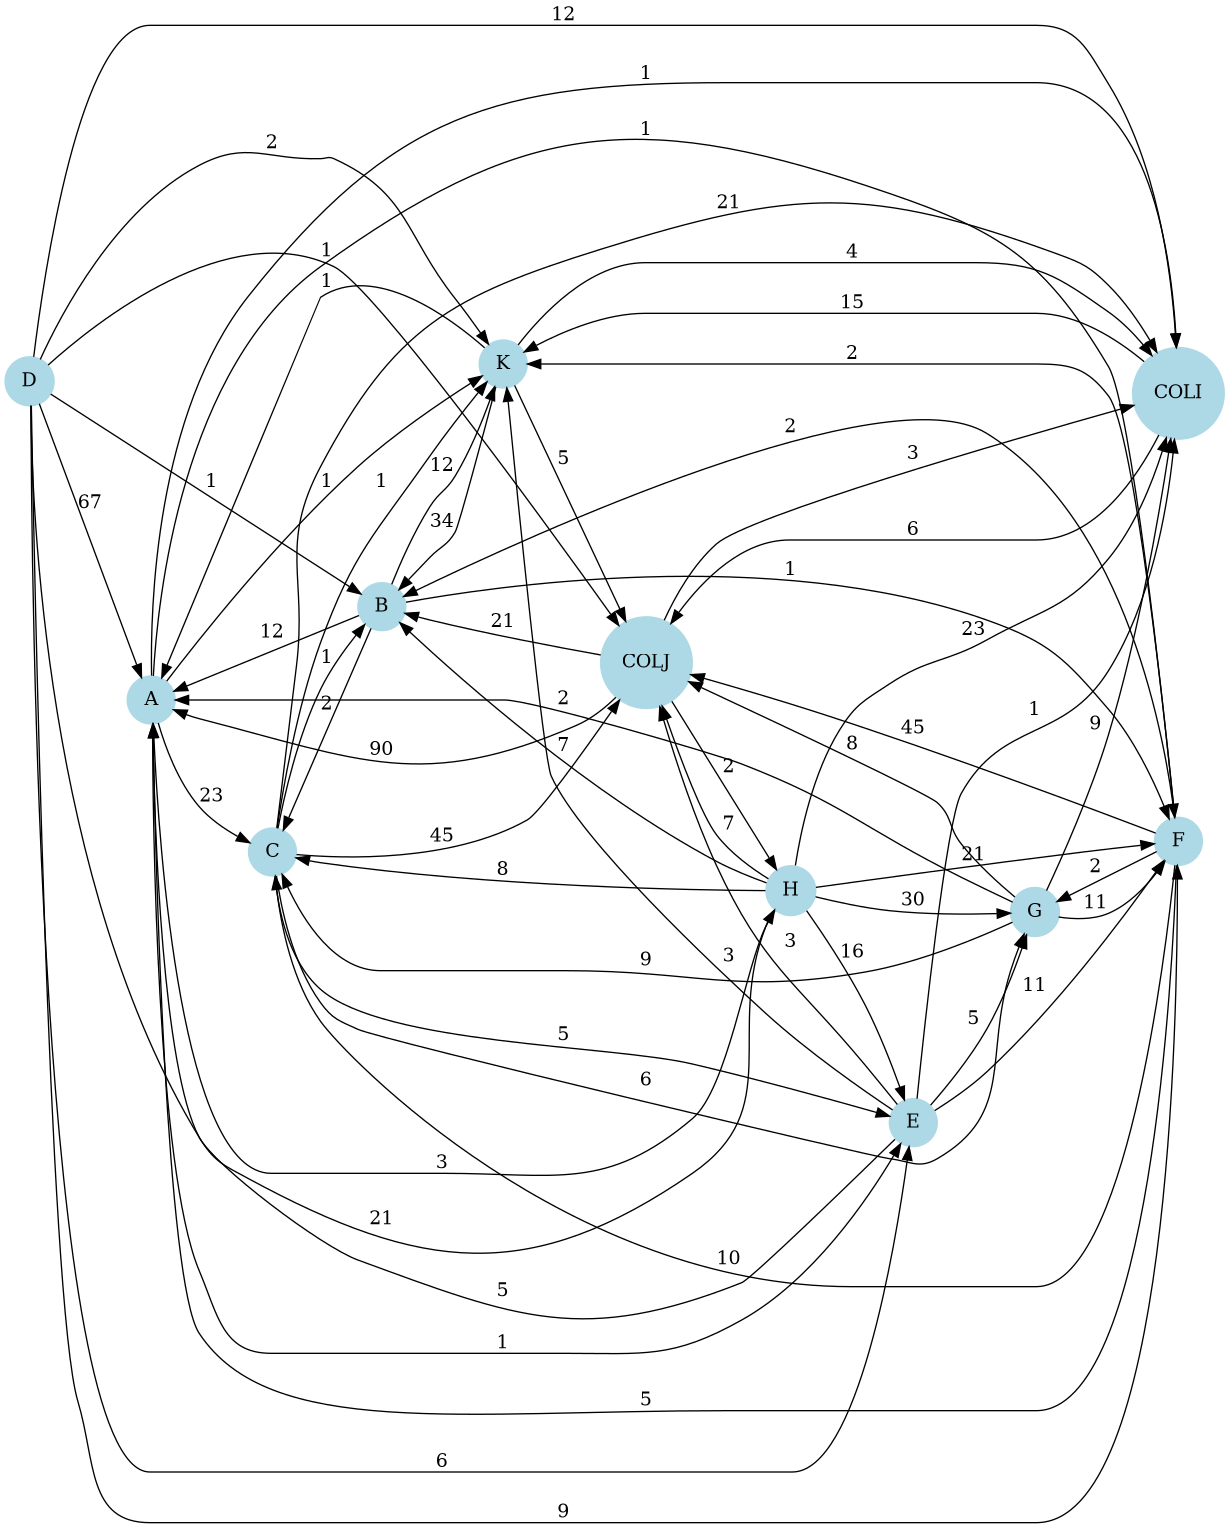
\includegraphics[width=0.5\textwidth,keepaspectratio]{grafo.png}
\caption{Representación del grafo original}
\end{figure}

\clearpage
\section{Procedimiento del Algoritmo}
\subsection{Matriz de Distancias Inicial D(0)}
\begin{table}[h!]
\centering
\begin{tabular}{|c|c|c|c|c|c|c|c|c|c|}
\hline
 & A & B & C & D & E & F & G & H & I \\\hline
A & 0 & $\infty$ & $\infty$ & $\infty$ & $\infty$ & $\infty$ & $\infty$ & $\infty$ & $\infty$ \\\hline
B & $\infty$ & 0 & $\infty$ & $\infty$ & $\infty$ & $\infty$ & $\infty$ & $\infty$ & $\infty$ \\\hline
C & $\infty$ & $\infty$ & 0 & $\infty$ & $\infty$ & $\infty$ & $\infty$ & $\infty$ & $\infty$ \\\hline
D & $\infty$ & $\infty$ & $\infty$ & 0 & $\infty$ & $\infty$ & $\infty$ & $\infty$ & $\infty$ \\\hline
E & $\infty$ & $\infty$ & $\infty$ & $\infty$ & 0 & $\infty$ & $\infty$ & $\infty$ & $\infty$ \\\hline
F & $\infty$ & $\infty$ & $\infty$ & $\infty$ & $\infty$ & 0 & $\infty$ & $\infty$ & $\infty$ \\\hline
G & $\infty$ & $\infty$ & $\infty$ & $\infty$ & $\infty$ & $\infty$ & 0 & $\infty$ & $\infty$ \\\hline
H & $\infty$ & $\infty$ & $\infty$ & $\infty$ & $\infty$ & $\infty$ & $\infty$ & 0 & $\infty$ \\\hline
I & $\infty$ & $\infty$ & $\infty$ & $\infty$ & $\infty$ & $\infty$ & $\infty$ & $\infty$ & 0 \\\hline
\end{tabular}
\caption{Matriz de distancias inicial D(0)}
\end{table}

\clearpage
\subsection{Matriz de Caminos Inicial P(0)}
\begin{table}[h!]
\centering
\begin{tabular}{|c|c|c|c|c|c|c|c|c|c|}
\hline
 & A & B & C & D & E & F & G & H & I \\\hline
A & - & - & - & - & - & - & - & - & - \\\hline
B & - & - & - & - & - & - & - & - & - \\\hline
C & - & - & - & - & - & - & - & - & - \\\hline
D & - & - & - & - & - & - & - & - & - \\\hline
E & - & - & - & - & - & - & - & - & - \\\hline
F & - & - & - & - & - & - & - & - & - \\\hline
G & - & - & - & - & - & - & - & - & - \\\hline
H & - & - & - & - & - & - & - & - & - \\\hline
I & - & - & - & - & - & - & - & - & - \\\hline
\end{tabular}
\caption{Matriz de caminos inicial P(0)}
\end{table}

\clearpage
\subsection{Iteraciones del Algoritmo}
\subsubsection{Iteración 1 (k = 1) - Nodo intermedio: A}
\paragraph{Matriz de Distancias D(1)}
\begin{table}[h!]
\centering
\begin{tabular}{|c|c|c|c|c|c|c|c|c|c|}
\hline
 & A & B & C & D & E & F & G & H & I \\\hline
A & 0 & $\infty$ & $\infty$ & $\infty$ & $\infty$ & $\infty$ & $\infty$ & $\infty$ & $\infty$ \\\hline
B & $\infty$ & 0 & $\infty$ & $\infty$ & $\infty$ & $\infty$ & $\infty$ & $\infty$ & $\infty$ \\\hline
C & $\infty$ & $\infty$ & 0 & $\infty$ & $\infty$ & $\infty$ & $\infty$ & $\infty$ & $\infty$ \\\hline
D & $\infty$ & $\infty$ & $\infty$ & 0 & $\infty$ & $\infty$ & $\infty$ & $\infty$ & $\infty$ \\\hline
E & $\infty$ & $\infty$ & $\infty$ & $\infty$ & 0 & $\infty$ & $\infty$ & $\infty$ & $\infty$ \\\hline
F & $\infty$ & $\infty$ & $\infty$ & $\infty$ & $\infty$ & 0 & $\infty$ & $\infty$ & $\infty$ \\\hline
G & $\infty$ & $\infty$ & $\infty$ & $\infty$ & $\infty$ & $\infty$ & 0 & $\infty$ & $\infty$ \\\hline
H & $\infty$ & $\infty$ & $\infty$ & $\infty$ & $\infty$ & $\infty$ & $\infty$ & 0 & $\infty$ \\\hline
I & $\infty$ & $\infty$ & $\infty$ & $\infty$ & $\infty$ & $\infty$ & $\infty$ & $\infty$ & 0 \\\hline
\end{tabular}
\caption{Matriz de distancias D(1) - Cambios resaltados en verde}
\end{table}

\paragraph{Matriz de Caminos P(1)}
\begin{table}[h!]
\centering
\begin{tabular}{|c|c|c|c|c|c|c|c|c|c|}
\hline
 & A & B & C & D & E & F & G & H & I \\\hline
A & - & - & - & - & - & - & - & - & - \\\hline
B & - & - & - & - & - & - & - & - & - \\\hline
C & - & - & - & - & - & - & - & - & - \\\hline
D & - & - & - & - & - & - & - & - & - \\\hline
E & - & - & - & - & - & - & - & - & - \\\hline
F & - & - & - & - & - & - & - & - & - \\\hline
G & - & - & - & - & - & - & - & - & - \\\hline
H & - & - & - & - & - & - & - & - & - \\\hline
I & - & - & - & - & - & - & - & - & - \\\hline
\end{tabular}
\caption{Matriz de caminos P(1) - Cambios resaltados en azul}
\end{table}

\subsubsection{Iteración 2 (k = 2) - Nodo intermedio: B}
\paragraph{Matriz de Distancias D(2)}
\begin{table}[h!]
\centering
\begin{tabular}{|c|c|c|c|c|c|c|c|c|c|}
\hline
 & A & B & C & D & E & F & G & H & I \\\hline
A & 0 & $\infty$ & $\infty$ & $\infty$ & $\infty$ & $\infty$ & $\infty$ & $\infty$ & $\infty$ \\\hline
B & $\infty$ & 0 & $\infty$ & $\infty$ & $\infty$ & $\infty$ & $\infty$ & $\infty$ & $\infty$ \\\hline
C & $\infty$ & $\infty$ & 0 & $\infty$ & $\infty$ & $\infty$ & $\infty$ & $\infty$ & $\infty$ \\\hline
D & $\infty$ & $\infty$ & $\infty$ & 0 & $\infty$ & $\infty$ & $\infty$ & $\infty$ & $\infty$ \\\hline
E & $\infty$ & $\infty$ & $\infty$ & $\infty$ & 0 & $\infty$ & $\infty$ & $\infty$ & $\infty$ \\\hline
F & $\infty$ & $\infty$ & $\infty$ & $\infty$ & $\infty$ & 0 & $\infty$ & $\infty$ & $\infty$ \\\hline
G & $\infty$ & $\infty$ & $\infty$ & $\infty$ & $\infty$ & $\infty$ & 0 & $\infty$ & $\infty$ \\\hline
H & $\infty$ & $\infty$ & $\infty$ & $\infty$ & $\infty$ & $\infty$ & $\infty$ & 0 & $\infty$ \\\hline
I & $\infty$ & $\infty$ & $\infty$ & $\infty$ & $\infty$ & $\infty$ & $\infty$ & $\infty$ & 0 \\\hline
\end{tabular}
\caption{Matriz de distancias D(2) - Cambios resaltados en verde}
\end{table}

\paragraph{Matriz de Caminos P(2)}
\begin{table}[h!]
\centering
\begin{tabular}{|c|c|c|c|c|c|c|c|c|c|}
\hline
 & A & B & C & D & E & F & G & H & I \\\hline
A & - & - & - & - & - & - & - & - & - \\\hline
B & - & - & - & - & - & - & - & - & - \\\hline
C & - & - & - & - & - & - & - & - & - \\\hline
D & - & - & - & - & - & - & - & - & - \\\hline
E & - & - & - & - & - & - & - & - & - \\\hline
F & - & - & - & - & - & - & - & - & - \\\hline
G & - & - & - & - & - & - & - & - & - \\\hline
H & - & - & - & - & - & - & - & - & - \\\hline
I & - & - & - & - & - & - & - & - & - \\\hline
\end{tabular}
\caption{Matriz de caminos P(2) - Cambios resaltados en azul}
\end{table}

\subsubsection{Iteración 3 (k = 3) - Nodo intermedio: C}
\paragraph{Matriz de Distancias D(3)}
\begin{table}[h!]
\centering
\begin{tabular}{|c|c|c|c|c|c|c|c|c|c|}
\hline
 & A & B & C & D & E & F & G & H & I \\\hline
A & 0 & $\infty$ & $\infty$ & $\infty$ & $\infty$ & $\infty$ & $\infty$ & $\infty$ & $\infty$ \\\hline
B & $\infty$ & 0 & $\infty$ & $\infty$ & $\infty$ & $\infty$ & $\infty$ & $\infty$ & $\infty$ \\\hline
C & $\infty$ & $\infty$ & 0 & $\infty$ & $\infty$ & $\infty$ & $\infty$ & $\infty$ & $\infty$ \\\hline
D & $\infty$ & $\infty$ & $\infty$ & 0 & $\infty$ & $\infty$ & $\infty$ & $\infty$ & $\infty$ \\\hline
E & $\infty$ & $\infty$ & $\infty$ & $\infty$ & 0 & $\infty$ & $\infty$ & $\infty$ & $\infty$ \\\hline
F & $\infty$ & $\infty$ & $\infty$ & $\infty$ & $\infty$ & 0 & $\infty$ & $\infty$ & $\infty$ \\\hline
G & $\infty$ & $\infty$ & $\infty$ & $\infty$ & $\infty$ & $\infty$ & 0 & $\infty$ & $\infty$ \\\hline
H & $\infty$ & $\infty$ & $\infty$ & $\infty$ & $\infty$ & $\infty$ & $\infty$ & 0 & $\infty$ \\\hline
I & $\infty$ & $\infty$ & $\infty$ & $\infty$ & $\infty$ & $\infty$ & $\infty$ & $\infty$ & 0 \\\hline
\end{tabular}
\caption{Matriz de distancias D(3) - Cambios resaltados en verde}
\end{table}

\paragraph{Matriz de Caminos P(3)}
\begin{table}[h!]
\centering
\begin{tabular}{|c|c|c|c|c|c|c|c|c|c|}
\hline
 & A & B & C & D & E & F & G & H & I \\\hline
A & - & - & - & - & - & - & - & - & - \\\hline
B & - & - & - & - & - & - & - & - & - \\\hline
C & - & - & - & - & - & - & - & - & - \\\hline
D & - & - & - & - & - & - & - & - & - \\\hline
E & - & - & - & - & - & - & - & - & - \\\hline
F & - & - & - & - & - & - & - & - & - \\\hline
G & - & - & - & - & - & - & - & - & - \\\hline
H & - & - & - & - & - & - & - & - & - \\\hline
I & - & - & - & - & - & - & - & - & - \\\hline
\end{tabular}
\caption{Matriz de caminos P(3) - Cambios resaltados en azul}
\end{table}

\subsubsection{Iteración 4 (k = 4) - Nodo intermedio: D}
\paragraph{Matriz de Distancias D(4)}
\begin{table}[h!]
\centering
\begin{tabular}{|c|c|c|c|c|c|c|c|c|c|}
\hline
 & A & B & C & D & E & F & G & H & I \\\hline
A & 0 & $\infty$ & $\infty$ & $\infty$ & $\infty$ & $\infty$ & $\infty$ & $\infty$ & $\infty$ \\\hline
B & $\infty$ & 0 & $\infty$ & $\infty$ & $\infty$ & $\infty$ & $\infty$ & $\infty$ & $\infty$ \\\hline
C & $\infty$ & $\infty$ & 0 & $\infty$ & $\infty$ & $\infty$ & $\infty$ & $\infty$ & $\infty$ \\\hline
D & $\infty$ & $\infty$ & $\infty$ & 0 & $\infty$ & $\infty$ & $\infty$ & $\infty$ & $\infty$ \\\hline
E & $\infty$ & $\infty$ & $\infty$ & $\infty$ & 0 & $\infty$ & $\infty$ & $\infty$ & $\infty$ \\\hline
F & $\infty$ & $\infty$ & $\infty$ & $\infty$ & $\infty$ & 0 & $\infty$ & $\infty$ & $\infty$ \\\hline
G & $\infty$ & $\infty$ & $\infty$ & $\infty$ & $\infty$ & $\infty$ & 0 & $\infty$ & $\infty$ \\\hline
H & $\infty$ & $\infty$ & $\infty$ & $\infty$ & $\infty$ & $\infty$ & $\infty$ & 0 & $\infty$ \\\hline
I & $\infty$ & $\infty$ & $\infty$ & $\infty$ & $\infty$ & $\infty$ & $\infty$ & $\infty$ & 0 \\\hline
\end{tabular}
\caption{Matriz de distancias D(4) - Cambios resaltados en verde}
\end{table}

\paragraph{Matriz de Caminos P(4)}
\begin{table}[h!]
\centering
\begin{tabular}{|c|c|c|c|c|c|c|c|c|c|}
\hline
 & A & B & C & D & E & F & G & H & I \\\hline
A & - & - & - & - & - & - & - & - & - \\\hline
B & - & - & - & - & - & - & - & - & - \\\hline
C & - & - & - & - & - & - & - & - & - \\\hline
D & - & - & - & - & - & - & - & - & - \\\hline
E & - & - & - & - & - & - & - & - & - \\\hline
F & - & - & - & - & - & - & - & - & - \\\hline
G & - & - & - & - & - & - & - & - & - \\\hline
H & - & - & - & - & - & - & - & - & - \\\hline
I & - & - & - & - & - & - & - & - & - \\\hline
\end{tabular}
\caption{Matriz de caminos P(4) - Cambios resaltados en azul}
\end{table}

\subsubsection{Iteración 5 (k = 5) - Nodo intermedio: E}
\paragraph{Matriz de Distancias D(5)}
\begin{table}[h!]
\centering
\begin{tabular}{|c|c|c|c|c|c|c|c|c|c|}
\hline
 & A & B & C & D & E & F & G & H & I \\\hline
A & 0 & $\infty$ & $\infty$ & $\infty$ & $\infty$ & $\infty$ & $\infty$ & $\infty$ & $\infty$ \\\hline
B & $\infty$ & 0 & $\infty$ & $\infty$ & $\infty$ & $\infty$ & $\infty$ & $\infty$ & $\infty$ \\\hline
C & $\infty$ & $\infty$ & 0 & $\infty$ & $\infty$ & $\infty$ & $\infty$ & $\infty$ & $\infty$ \\\hline
D & $\infty$ & $\infty$ & $\infty$ & 0 & $\infty$ & $\infty$ & $\infty$ & $\infty$ & $\infty$ \\\hline
E & $\infty$ & $\infty$ & $\infty$ & $\infty$ & 0 & $\infty$ & $\infty$ & $\infty$ & $\infty$ \\\hline
F & $\infty$ & $\infty$ & $\infty$ & $\infty$ & $\infty$ & 0 & $\infty$ & $\infty$ & $\infty$ \\\hline
G & $\infty$ & $\infty$ & $\infty$ & $\infty$ & $\infty$ & $\infty$ & 0 & $\infty$ & $\infty$ \\\hline
H & $\infty$ & $\infty$ & $\infty$ & $\infty$ & $\infty$ & $\infty$ & $\infty$ & 0 & $\infty$ \\\hline
I & $\infty$ & $\infty$ & $\infty$ & $\infty$ & $\infty$ & $\infty$ & $\infty$ & $\infty$ & 0 \\\hline
\end{tabular}
\caption{Matriz de distancias D(5) - Cambios resaltados en verde}
\end{table}

\paragraph{Matriz de Caminos P(5)}
\begin{table}[h!]
\centering
\begin{tabular}{|c|c|c|c|c|c|c|c|c|c|}
\hline
 & A & B & C & D & E & F & G & H & I \\\hline
A & - & - & - & - & - & - & - & - & - \\\hline
B & - & - & - & - & - & - & - & - & - \\\hline
C & - & - & - & - & - & - & - & - & - \\\hline
D & - & - & - & - & - & - & - & - & - \\\hline
E & - & - & - & - & - & - & - & - & - \\\hline
F & - & - & - & - & - & - & - & - & - \\\hline
G & - & - & - & - & - & - & - & - & - \\\hline
H & - & - & - & - & - & - & - & - & - \\\hline
I & - & - & - & - & - & - & - & - & - \\\hline
\end{tabular}
\caption{Matriz de caminos P(5) - Cambios resaltados en azul}
\end{table}

\subsubsection{Iteración 6 (k = 6) - Nodo intermedio: F}
\paragraph{Matriz de Distancias D(6)}
\begin{table}[h!]
\centering
\begin{tabular}{|c|c|c|c|c|c|c|c|c|c|}
\hline
 & A & B & C & D & E & F & G & H & I \\\hline
A & 0 & $\infty$ & $\infty$ & $\infty$ & $\infty$ & $\infty$ & $\infty$ & $\infty$ & $\infty$ \\\hline
B & $\infty$ & 0 & $\infty$ & $\infty$ & $\infty$ & $\infty$ & $\infty$ & $\infty$ & $\infty$ \\\hline
C & $\infty$ & $\infty$ & 0 & $\infty$ & $\infty$ & $\infty$ & $\infty$ & $\infty$ & $\infty$ \\\hline
D & $\infty$ & $\infty$ & $\infty$ & 0 & $\infty$ & $\infty$ & $\infty$ & $\infty$ & $\infty$ \\\hline
E & $\infty$ & $\infty$ & $\infty$ & $\infty$ & 0 & $\infty$ & $\infty$ & $\infty$ & $\infty$ \\\hline
F & $\infty$ & $\infty$ & $\infty$ & $\infty$ & $\infty$ & 0 & $\infty$ & $\infty$ & $\infty$ \\\hline
G & $\infty$ & $\infty$ & $\infty$ & $\infty$ & $\infty$ & $\infty$ & 0 & $\infty$ & $\infty$ \\\hline
H & $\infty$ & $\infty$ & $\infty$ & $\infty$ & $\infty$ & $\infty$ & $\infty$ & 0 & $\infty$ \\\hline
I & $\infty$ & $\infty$ & $\infty$ & $\infty$ & $\infty$ & $\infty$ & $\infty$ & $\infty$ & 0 \\\hline
\end{tabular}
\caption{Matriz de distancias D(6) - Cambios resaltados en verde}
\end{table}

\paragraph{Matriz de Caminos P(6)}
\begin{table}[h!]
\centering
\begin{tabular}{|c|c|c|c|c|c|c|c|c|c|}
\hline
 & A & B & C & D & E & F & G & H & I \\\hline
A & - & - & - & - & - & - & - & - & - \\\hline
B & - & - & - & - & - & - & - & - & - \\\hline
C & - & - & - & - & - & - & - & - & - \\\hline
D & - & - & - & - & - & - & - & - & - \\\hline
E & - & - & - & - & - & - & - & - & - \\\hline
F & - & - & - & - & - & - & - & - & - \\\hline
G & - & - & - & - & - & - & - & - & - \\\hline
H & - & - & - & - & - & - & - & - & - \\\hline
I & - & - & - & - & - & - & - & - & - \\\hline
\end{tabular}
\caption{Matriz de caminos P(6) - Cambios resaltados en azul}
\end{table}

\subsubsection{Iteración 7 (k = 7) - Nodo intermedio: G}
\paragraph{Matriz de Distancias D(7)}
\begin{table}[h!]
\centering
\begin{tabular}{|c|c|c|c|c|c|c|c|c|c|}
\hline
 & A & B & C & D & E & F & G & H & I \\\hline
A & 0 & $\infty$ & $\infty$ & $\infty$ & $\infty$ & $\infty$ & $\infty$ & $\infty$ & $\infty$ \\\hline
B & $\infty$ & 0 & $\infty$ & $\infty$ & $\infty$ & $\infty$ & $\infty$ & $\infty$ & $\infty$ \\\hline
C & $\infty$ & $\infty$ & 0 & $\infty$ & $\infty$ & $\infty$ & $\infty$ & $\infty$ & $\infty$ \\\hline
D & $\infty$ & $\infty$ & $\infty$ & 0 & $\infty$ & $\infty$ & $\infty$ & $\infty$ & $\infty$ \\\hline
E & $\infty$ & $\infty$ & $\infty$ & $\infty$ & 0 & $\infty$ & $\infty$ & $\infty$ & $\infty$ \\\hline
F & $\infty$ & $\infty$ & $\infty$ & $\infty$ & $\infty$ & 0 & $\infty$ & $\infty$ & $\infty$ \\\hline
G & $\infty$ & $\infty$ & $\infty$ & $\infty$ & $\infty$ & $\infty$ & 0 & $\infty$ & $\infty$ \\\hline
H & $\infty$ & $\infty$ & $\infty$ & $\infty$ & $\infty$ & $\infty$ & $\infty$ & 0 & $\infty$ \\\hline
I & $\infty$ & $\infty$ & $\infty$ & $\infty$ & $\infty$ & $\infty$ & $\infty$ & $\infty$ & 0 \\\hline
\end{tabular}
\caption{Matriz de distancias D(7) - Cambios resaltados en verde}
\end{table}

\paragraph{Matriz de Caminos P(7)}
\begin{table}[h!]
\centering
\begin{tabular}{|c|c|c|c|c|c|c|c|c|c|}
\hline
 & A & B & C & D & E & F & G & H & I \\\hline
A & - & - & - & - & - & - & - & - & - \\\hline
B & - & - & - & - & - & - & - & - & - \\\hline
C & - & - & - & - & - & - & - & - & - \\\hline
D & - & - & - & - & - & - & - & - & - \\\hline
E & - & - & - & - & - & - & - & - & - \\\hline
F & - & - & - & - & - & - & - & - & - \\\hline
G & - & - & - & - & - & - & - & - & - \\\hline
H & - & - & - & - & - & - & - & - & - \\\hline
I & - & - & - & - & - & - & - & - & - \\\hline
\end{tabular}
\caption{Matriz de caminos P(7) - Cambios resaltados en azul}
\end{table}

\subsubsection{Iteración 8 (k = 8) - Nodo intermedio: H}
\paragraph{Matriz de Distancias D(8)}
\begin{table}[h!]
\centering
\begin{tabular}{|c|c|c|c|c|c|c|c|c|c|}
\hline
 & A & B & C & D & E & F & G & H & I \\\hline
A & 0 & $\infty$ & $\infty$ & $\infty$ & $\infty$ & $\infty$ & $\infty$ & $\infty$ & $\infty$ \\\hline
B & $\infty$ & 0 & $\infty$ & $\infty$ & $\infty$ & $\infty$ & $\infty$ & $\infty$ & $\infty$ \\\hline
C & $\infty$ & $\infty$ & 0 & $\infty$ & $\infty$ & $\infty$ & $\infty$ & $\infty$ & $\infty$ \\\hline
D & $\infty$ & $\infty$ & $\infty$ & 0 & $\infty$ & $\infty$ & $\infty$ & $\infty$ & $\infty$ \\\hline
E & $\infty$ & $\infty$ & $\infty$ & $\infty$ & 0 & $\infty$ & $\infty$ & $\infty$ & $\infty$ \\\hline
F & $\infty$ & $\infty$ & $\infty$ & $\infty$ & $\infty$ & 0 & $\infty$ & $\infty$ & $\infty$ \\\hline
G & $\infty$ & $\infty$ & $\infty$ & $\infty$ & $\infty$ & $\infty$ & 0 & $\infty$ & $\infty$ \\\hline
H & $\infty$ & $\infty$ & $\infty$ & $\infty$ & $\infty$ & $\infty$ & $\infty$ & 0 & $\infty$ \\\hline
I & $\infty$ & $\infty$ & $\infty$ & $\infty$ & $\infty$ & $\infty$ & $\infty$ & $\infty$ & 0 \\\hline
\end{tabular}
\caption{Matriz de distancias D(8) - Cambios resaltados en verde}
\end{table}

\paragraph{Matriz de Caminos P(8)}
\begin{table}[h!]
\centering
\begin{tabular}{|c|c|c|c|c|c|c|c|c|c|}
\hline
 & A & B & C & D & E & F & G & H & I \\\hline
A & - & - & - & - & - & - & - & - & - \\\hline
B & - & - & - & - & - & - & - & - & - \\\hline
C & - & - & - & - & - & - & - & - & - \\\hline
D & - & - & - & - & - & - & - & - & - \\\hline
E & - & - & - & - & - & - & - & - & - \\\hline
F & - & - & - & - & - & - & - & - & - \\\hline
G & - & - & - & - & - & - & - & - & - \\\hline
H & - & - & - & - & - & - & - & - & - \\\hline
I & - & - & - & - & - & - & - & - & - \\\hline
\end{tabular}
\caption{Matriz de caminos P(8) - Cambios resaltados en azul}
\end{table}

\subsubsection{Iteración 9 (k = 9) - Nodo intermedio: I}
\paragraph{Matriz de Distancias D(9)}
\begin{table}[h!]
\centering
\begin{tabular}{|c|c|c|c|c|c|c|c|c|c|}
\hline
 & A & B & C & D & E & F & G & H & I \\\hline
A & 0 & $\infty$ & $\infty$ & $\infty$ & $\infty$ & $\infty$ & $\infty$ & $\infty$ & $\infty$ \\\hline
B & $\infty$ & 0 & $\infty$ & $\infty$ & $\infty$ & $\infty$ & $\infty$ & $\infty$ & $\infty$ \\\hline
C & $\infty$ & $\infty$ & 0 & $\infty$ & $\infty$ & $\infty$ & $\infty$ & $\infty$ & $\infty$ \\\hline
D & $\infty$ & $\infty$ & $\infty$ & 0 & $\infty$ & $\infty$ & $\infty$ & $\infty$ & $\infty$ \\\hline
E & $\infty$ & $\infty$ & $\infty$ & $\infty$ & 0 & $\infty$ & $\infty$ & $\infty$ & $\infty$ \\\hline
F & $\infty$ & $\infty$ & $\infty$ & $\infty$ & $\infty$ & 0 & $\infty$ & $\infty$ & $\infty$ \\\hline
G & $\infty$ & $\infty$ & $\infty$ & $\infty$ & $\infty$ & $\infty$ & 0 & $\infty$ & $\infty$ \\\hline
H & $\infty$ & $\infty$ & $\infty$ & $\infty$ & $\infty$ & $\infty$ & $\infty$ & 0 & $\infty$ \\\hline
I & $\infty$ & $\infty$ & $\infty$ & $\infty$ & $\infty$ & $\infty$ & $\infty$ & $\infty$ & 0 \\\hline
\end{tabular}
\caption{Matriz de distancias D(9) - Cambios resaltados en verde}
\end{table}

\paragraph{Matriz de Caminos P(9)}
\begin{table}[h!]
\centering
\begin{tabular}{|c|c|c|c|c|c|c|c|c|c|}
\hline
 & A & B & C & D & E & F & G & H & I \\\hline
A & - & - & - & - & - & - & - & - & - \\\hline
B & - & - & - & - & - & - & - & - & - \\\hline
C & - & - & - & - & - & - & - & - & - \\\hline
D & - & - & - & - & - & - & - & - & - \\\hline
E & - & - & - & - & - & - & - & - & - \\\hline
F & - & - & - & - & - & - & - & - & - \\\hline
G & - & - & - & - & - & - & - & - & - \\\hline
H & - & - & - & - & - & - & - & - & - \\\hline
I & - & - & - & - & - & - & - & - & - \\\hline
\end{tabular}
\caption{Matriz de caminos P(9) - Cambios resaltados en azul}
\end{table}

\clearpage
\section{Resultados Finales}
\subsection{Matriz de Distancias Final D(9)}
\begin{table}[h!]
\centering
\begin{tabular}{|c|c|c|c|c|c|c|c|c|c|}
\hline
 & A & B & C & D & E & F & G & H & I \\\hline
A & 0 & $\infty$ & $\infty$ & $\infty$ & $\infty$ & $\infty$ & $\infty$ & $\infty$ & $\infty$ \\\hline
B & $\infty$ & 0 & $\infty$ & $\infty$ & $\infty$ & $\infty$ & $\infty$ & $\infty$ & $\infty$ \\\hline
C & $\infty$ & $\infty$ & 0 & $\infty$ & $\infty$ & $\infty$ & $\infty$ & $\infty$ & $\infty$ \\\hline
D & $\infty$ & $\infty$ & $\infty$ & 0 & $\infty$ & $\infty$ & $\infty$ & $\infty$ & $\infty$ \\\hline
E & $\infty$ & $\infty$ & $\infty$ & $\infty$ & 0 & $\infty$ & $\infty$ & $\infty$ & $\infty$ \\\hline
F & $\infty$ & $\infty$ & $\infty$ & $\infty$ & $\infty$ & 0 & $\infty$ & $\infty$ & $\infty$ \\\hline
G & $\infty$ & $\infty$ & $\infty$ & $\infty$ & $\infty$ & $\infty$ & 0 & $\infty$ & $\infty$ \\\hline
H & $\infty$ & $\infty$ & $\infty$ & $\infty$ & $\infty$ & $\infty$ & $\infty$ & 0 & $\infty$ \\\hline
I & $\infty$ & $\infty$ & $\infty$ & $\infty$ & $\infty$ & $\infty$ & $\infty$ & $\infty$ & 0 \\\hline
\end{tabular}
\caption{Matriz de distancias final D(9)}
\end{table}

\clearpage
\subsection{Matriz de Caminos Final P(9)}
\begin{table}[h!]
\centering
\begin{tabular}{|c|c|c|c|c|c|c|c|c|c|}
\hline
 & A & B & C & D & E & F & G & H & I \\\hline
A & - & - & - & - & - & - & - & - & - \\\hline
B & - & - & - & - & - & - & - & - & - \\\hline
C & - & - & - & - & - & - & - & - & - \\\hline
D & - & - & - & - & - & - & - & - & - \\\hline
E & - & - & - & - & - & - & - & - & - \\\hline
F & - & - & - & - & - & - & - & - & - \\\hline
G & - & - & - & - & - & - & - & - & - \\\hline
H & - & - & - & - & - & - & - & - & - \\\hline
I & - & - & - & - & - & - & - & - & - \\\hline
\end{tabular}
\caption{Matriz de caminos final P(9)}
\end{table}

\clearpage
\subsection{Rutas Óptimas}
\begin{itemize}
\item No hay rutas válidas entre los nodos.
\end{itemize}
\end{document}
